\documentclass[../../main.tex]{subfiles}
\begin{document}

\begin{figure}
    \centering
    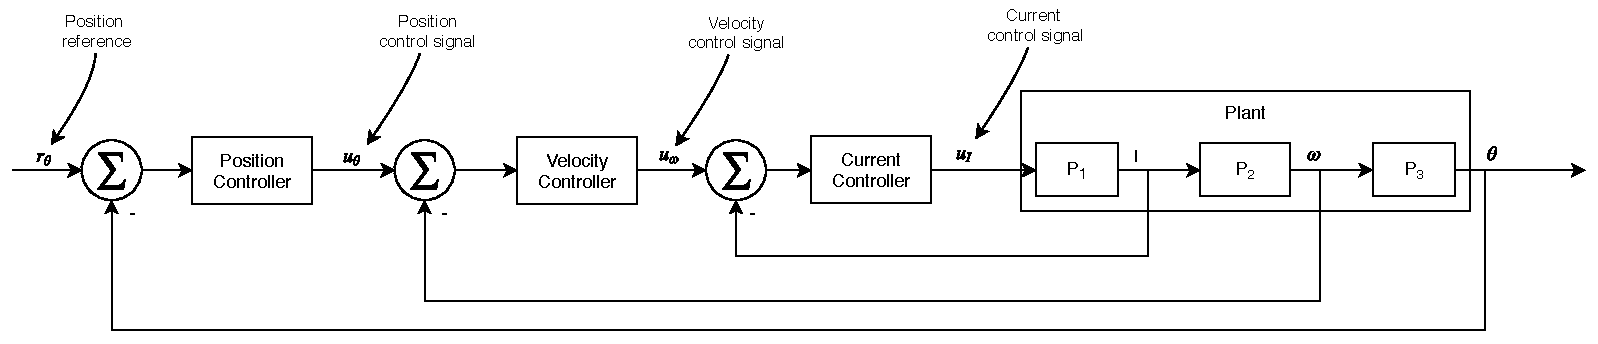
\includegraphics[width = 0.9\textwidth]{Images/AnalysisImages/controllerDiagram.pdf}
    \caption{Caption}
    \label{fig:system_diagram}
\end{figure}

\section{Open loop transferfunction for the current controller}

\begin{equation}
    I = u_{I} \cdot P_1\cdot k_{cc}
\end{equation}
\begin{equation}
    \frac{I}{u_{I}} = P_1\cdot K_{cc} 
\end{equation}
     




\section{The closed loop transferfunction for the current control}

The closed loop transferfunction is derived from the two equtions: 
\begin{equation}
    I = u_i \cdot P_1 \quad \quad
    u_i = (u_{\omega}-I)\cdot k_{cc}
\end{equation}

The equations are combined to two derive a expression for the tranferfunction. 

\begin{equation}
    I = (u_{\omega}-I)\cdot k_{cc}\cdot P_1
\end{equation}
\begin{equation}
    I = \frac{u_{\omega}\cdot K_{cc}\cdot P_1}{1+K_{cc}\cdot P_1}
\end{equation}
\begin{equation}
    \frac{I}{u_{\omega}} =  \frac{ K_{cc}\cdot P_1}{1+K_{cc}\cdot P_1}
\end{equation}

Where $K_{cc}$ is the PID used for the control of the current. $K_{cc}$  is equal to $(K_{pcc} e(t) + K_{icc}\int_0^t e(t) + K_{dcc}\frac{de(t)}{dt})$
\end{document}